\documentclass[12pt,a4paper]{article}
\usepackage[utf8]{inputenc}
\usepackage[spanish,es-tabla]{babel}
\usepackage{geometry}
\usepackage{graphicx}
\usepackage{multirow}
\usepackage{tabularx}
\usepackage{mathptmx}
\usepackage{fancyhdr}
\usepackage{array}
\usepackage[table]{xcolor}
\usepackage{titlesec}
\usepackage{setspace}
\usepackage{microtype}
\usepackage{lastpage}
\usepackage{booktabs}
\usepackage{enumitem}
\usepackage{amsmath}
\usepackage{amsfonts}
\usepackage{amssymb}

\usepackage{float}
\usepackage{placeins}
\usepackage{tikz}
\usepackage{pgfplots}
\pgfplotsset{compat=1.17}
\usetikzlibrary{arrows.meta,positioning,shapes.geometric,calc}

\graphicspath{{images/}{../images/}{./}}

\geometry{
    top=4.7cm,
    bottom=2.5cm,
    left=2.5cm,
    right=2.5cm,
    headheight=3.9cm,
    headsep=0.4cm
}

\setstretch{1.15}
\setlength{\parindent}{0pt}
\setlength{\parskip}{0.45em}
\setlength{\tabcolsep}{4pt}

\titleformat{\section}
  {\normalfont\fontsize{12}{14.5}\bfseries}{\thesection.}{0.6em}{\uppercase}
\titlespacing*{\section}
  {0pt}{1.8ex plus 0.4ex minus 0.2ex}{0.6ex plus 0.2ex}

\titleformat{\subsection}
  {\normalfont\fontsize{11.5}{13.5}\bfseries}{\thesubsection.}{0.5em}{}
\titlespacing*{\subsection}
  {0pt}{1.4ex plus 0.3ex minus 0.1ex}{0.4ex plus 0.1ex}

\titleformat{\subsubsection}
  {\normalfont\fontsize{10.5}{12.5}\bfseries\itshape}{\thesubsubsection.}{0.4em}{}
\titlespacing*{\subsubsection}
  {0pt}{1.1ex plus 0.2ex minus 0.1ex}{0.3ex plus 0.1ex}

\newcolumntype{Y}{>{\centering\arraybackslash}X}
\newcolumntype{L}{>{\raggedright\arraybackslash}X}
\newcolumntype{C}{>{\centering\arraybackslash}X}

\definecolor{headerblue}{RGB}{26, 54, 93}
\definecolor{darkblue}{RGB}{43, 108, 176}
\definecolor{lightgraybg}{RGB}{248, 248, 248}
\definecolor{tableheader}{RGB}{232, 238, 246}
\definecolor{navyheader}{RGB}{0, 32, 96}
\definecolor{lineblue}{RGB}{0, 102, 204}
\definecolor{areablue}{RGB}{220, 236, 252}
\definecolor{lcsred}{RGB}{217, 56, 41}
\definecolor{lcigreen}{RGB}{46, 125, 50}
\definecolor{lciorange}{RGB}{230, 81, 0}
\definecolor{ishikawared}{RGB}{160, 0, 0}

\tikzset{
    catbox/.style={draw, fill=tableheader, font=\footnotesize\bfseries, minimum width=2.8cm, minimum height=0.65cm, align=center},
    efectobox/.style={draw=ishikawared!90!black, line width=1.2pt, fill=ishikawared, text=white, font=\small\bfseries, align=center, inner sep=6pt, text width=3.8cm},
    causetext/.style={font=\scriptsize, align=right, text=black!90}
}

\newcommand{\docCodigo}{TI-SIGE-ENT-F3-008}
\newcommand{\docVersion}{1.0}
\newcommand{\docProceso}{GESTIÓN DE CALIDAD Y CONTROL DE HITOS / HITO 3 WIZARD}
\newcommand{\docElaboracion}{22/09/2026}
\newcommand{\docRevision}{22/09/2026}
\newcommand{\docTitulo}{HITO 3: SPRINT 2 REVIEW: WIZARD}
\newcommand{\docOrganizacion}{FACULTAD DE INGENIERÍA EN SISTEMAS, ELECTRÓNICA E INDUSTRIAL}
\newcommand{\docSubOrganizacion}{CARRERA DE INGENIERÍA DE SOFTWARE}

\newcommand{\encabezadofrecuente}{%
    \renewcommand{\arraystretch}{1.15}%
    \noindent\makebox[\textwidth][c]{%
    \begin{tabularx}{\textwidth}{|>{\centering\arraybackslash}m{2.8cm}|Y|>{\centering\arraybackslash}m{4.8cm}|}
        \hline
        \multirow{4}{2.8cm}{\centering\raisebox{-1.15cm}{
\includegraphics[width=2.5cm,height=2.0cm,keepaspectratio]{images/logo.png}}}
        & \textbf{\fontsize{9}{11}\selectfont \docOrganizacion} 
        & \textbf{\fontsize{8}{10}\selectfont CÓDIGO:} \fontsize{8}{10}\selectfont \docCodigo \\
        \cline{3-3}
        & \textbf{\fontsize{8.5}{10.5}\selectfont \docSubOrganizacion} 
        & \textbf{\fontsize{8}{10}\selectfont VERSIÓN:} \fontsize{8}{10}\selectfont \docVersion \\
        \cline{2-3}
        & \textbf{\fontsize{8}{10}\selectfont PROCESO:} \fontsize{8}{10}\selectfont \docProceso 
        & \textbf{\fontsize{8}{10}\selectfont ELABORACIÓN:} \fontsize{8}{10}\selectfont \docElaboracion \\
        \cline{2-3}
        & \textbf{\fontsize{8.5}{10.5}\selectfont \docTitulo} 
        & \textbf{\fontsize{8}{10}\selectfont ÚLTIMA REVISIÓN:} \fontsize{8}{10}\selectfont \docRevision \\
        \hline
    \end{tabularx}%
    }%
}

\pagestyle{fancy}
\fancyhf{}
\fancyhead[C]{\encabezadofrecuente}
\fancyfoot[C]{\fontsize{10}{12}\selectfont Página \thepage\ de \pageref{LastPage}}
\renewcommand{\headrulewidth}{0pt}

\begin{document}

\noindent{\fontsize{10.5}{12.5}\selectfont \textbf{Integrantes:} Heidi Villavicencio \quad$\vert$\quad Steeven Toala \quad$\vert$\quad Nixon Hurtado \quad$\vert$\quad Andrea Vásquez}

\vspace{0.25cm}

\section{Título}
\textbf{Denominación Oficial del Entregable:} HITO 3: Sprint 2 Review: Wizard y Persistencia Operativa -- Código EDT: 3.8

\section{Introducción}
La culminación del Sprint 2 de desarrollo marca el primer punto de inspección funcional del software operativo del sistema SIGE. En este hito intermedio (\textit{Sprint Review 2}) se audita la integración plena entre la capa de interfaz de usuario guiada por pestañas (\texttt{PlanEditorWizard}), el editor enriquecido con autoguardado (\texttt{RichTextEditor}) y los endpoints de persistencia transaccional en PostgreSQL 18. El presente informe formaliza los resultados de la sesión de demostración ante el Docente Evaluador, validando que el cuerpo docente cuenta con una solución operativa capaz de registrar y custodiar planes de trabajo institucionales en tiempo real.

\section{Objetivo}
\subsection{Objetivo General}
Auditar, demostrar y legalizar el cumplimiento de los objetivos y criterios de aceptación del Sprint 2 del sistema SIGE, aprobando el Hito 3 de la EDT.
\subsection{Objetivos Específicos}
\begin{itemize}[leftmargin=1.5em, itemsep=2pt]
    \item Demostrar el flujo funcional completo desde la autenticación hasta el guardado de secciones enriquecidas.
    \item Verificar la persistencia efectiva y no volátil en el contenedor PostgreSQL 18.
    \item Emitir el acta oficial de aprobación del Sprint 2 autorizando el inicio del Sprint 3.
\end{itemize}

\section{Alcance}
\subsection{Límites del Entregable (In-Scope)}
\begin{itemize}[leftmargin=1.5em, itemsep=2pt]
    \item Auditoría funcional de las tareas EDT 3.4 a 3.7.
    \item Verificación del 100\% de criterios de aceptación de las Historias de Usuario US-05 a US-10.
\end{itemize}
\subsection{Exclusiones (Out-of-Scope)}
\begin{itemize}[leftmargin=1.5em, itemsep=2pt]
    \item Carga física de evidencias en storage MinIO S3 (objeto del Sprint 3).
\end{itemize}

\section{Definiciones}
\begin{itemize}[leftmargin=1.5em, itemsep=2pt]
    \item \textbf{Sprint Review:} Ceremonia Scrum donde el equipo de desarrollo presenta los incrementos potencialmente desplegables a los interesados.
    \item \textbf{Incremento de Software:} Conjunto de ítems del Product Backlog completados durante un Sprint que cumplen la Definición de Terminado (\textit{DoD}).
    \item \textbf{Definition of Done (DoD):} Criterio consensuado que certifica que un componente está codificado, probado, integrado y documentado.
\end{itemize}

\section{Responsabilidades}
\begin{itemize}[leftmargin=1.5em, itemsep=2pt]
    \item \textbf{Steeven Toala (Líder Técnico / Scrum Master):} Dirección de la demostración funcional y sustentación técnica del Sprint 2.
    \item \textbf{Heidi Villavicencio (UI / Calidad):} Verificación de la fidelidad visual y ergonomía de usuario.
    \item \textbf{Andrea Vásquez / Nixon Hurtado (Desarrollo):} Pruebas de integración de componentes y persistencia.
    \item \textbf{Ing. Paulo Torres (Docente Evaluador):} Aprobación y legalización formal del Hito 3.
\end{itemize}

\section{Normativa Legal y Técnica}
\subsection{Marco Legal Ecuatoriano}
\begin{itemize}[leftmargin=1.5em, itemsep=2pt]
    \item \textbf{Ley Orgánica de Educación Superior (LOES), Art. 122 y 149:} Eficiencia y confiabilidad técnica en la digitalización de procesos universitarios.
\end{itemize}
\subsection{Normas Técnicas Internacionales}
\begin{itemize}[leftmargin=1.5em, itemsep=2pt]
    \item \textbf{Scrum Guide (Schwaber \& Sutherland):} Principios de inspección y adaptación continua.
    \item \textbf{ISO 9001:2015, Cláusula 8.3.4:} Controles del diseño y desarrollo para verificar que las salidas satisfagan los requisitos de entrada.
\end{itemize}

\section{Método, Políticas y Contenidos}
\subsection{Enfoque Metodológico}
Se ejecutó una sesión formal de revisión de Sprint siguiendo la metodología Scrum-XP. Se utilizó un escenario de prueba fáctico con un usuario docente titular de FISEI. Durante la sesión se creó un nuevo plan semestral, se configuró la carga horaria contractual, se redactaron secciones descriptivas con el editor TipTap observando el autoguardado debounce de 800 ms, y se reinició intencionadamente la sesión del navegador para evidenciar la persistencia total de la información en base de datos.

\subsection{Políticas de Calidad de Aprobación de Sprint}
\begin{enumerate}[leftmargin=1.5em, itemsep=2pt]
    \item \textbf{Política de Cero Bloqueadores en DoD:} Ninguna historia de usuario puede darse por aprobada si presenta defectos funcionales críticos abiertos.
    \item \textbf{Política de Persistencia Comprobada:} Toda demostración debe validar la consulta directa contra PostgreSQL 18 confirmando la no volatilidad de los datos.
    \item \textbf{Política de Registro de Observaciones:} Cualquier recomendación formulada por el Docente Evaluador se incorpora al Product Backlog del Sprint 3.
\end{enumerate}

\begin{figure}[H]
    \centering
    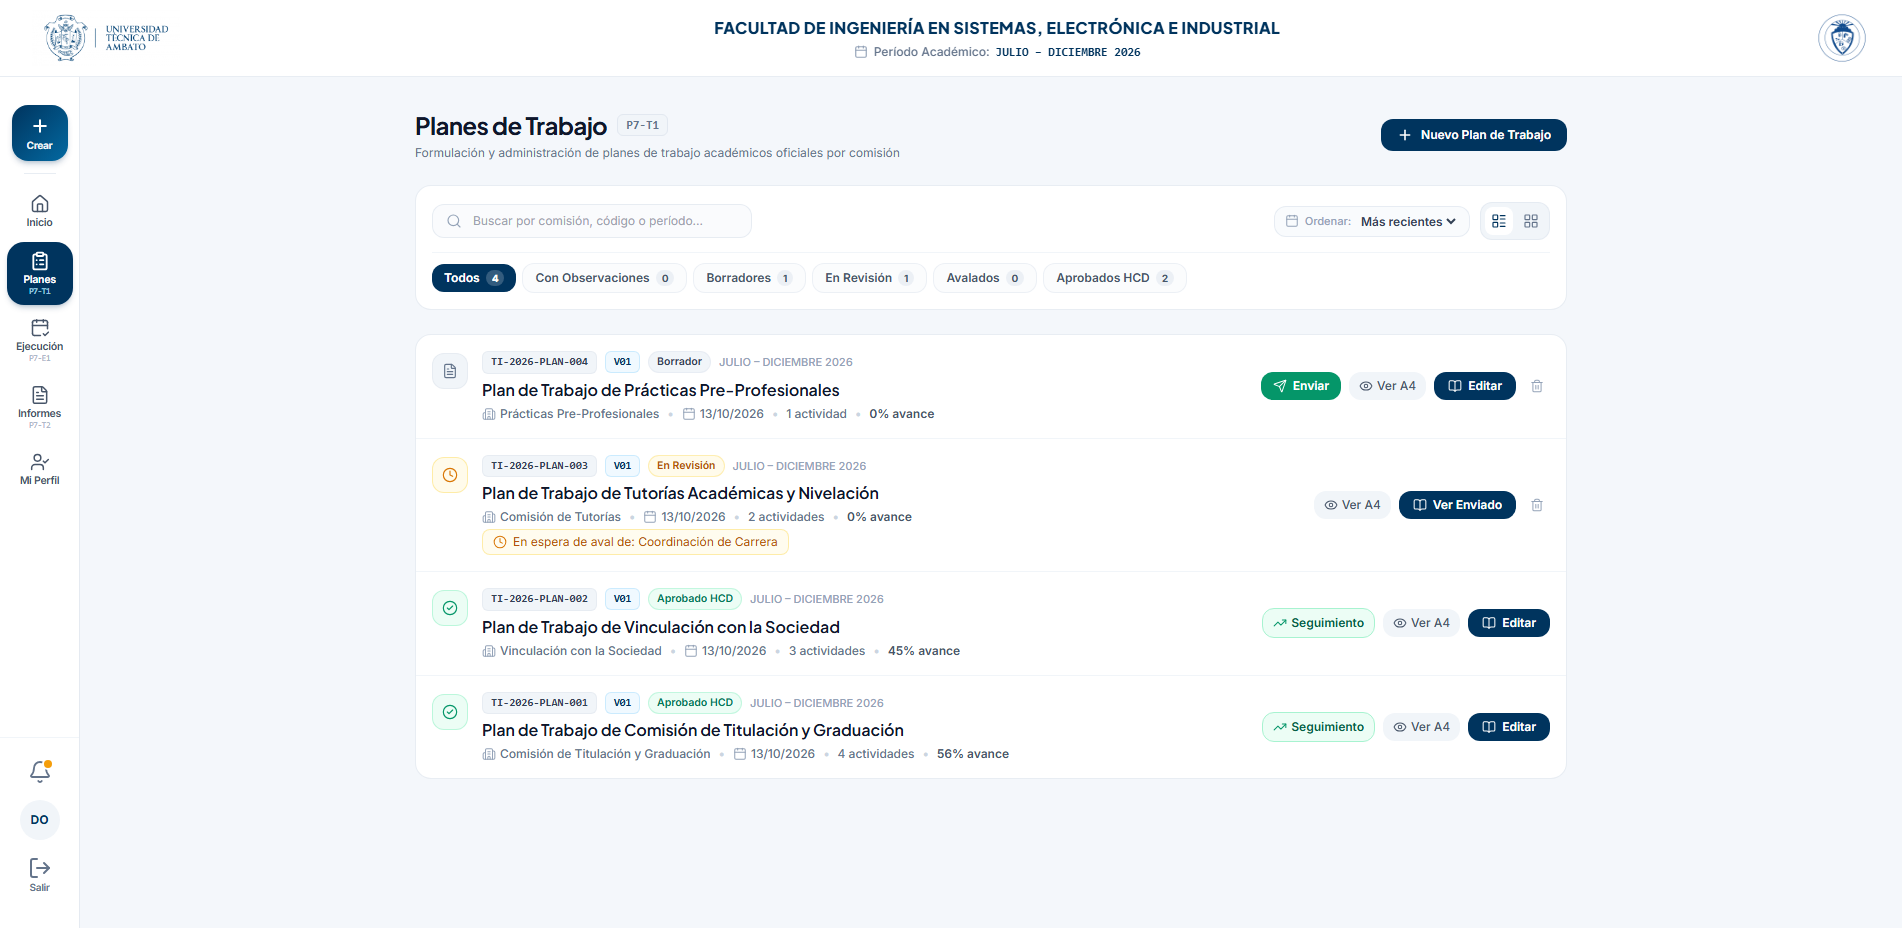
\includegraphics[width=0.88\textwidth,height=5.8cm,keepaspectratio]{images/sige_bandeja_planes.png}
    \caption{Captura Real de la Demostración de Planes Persistidos en la Base de Datos al Hito 3.}
    \label{fig:hito3_demo}
\end{figure}
\FloatBarrier

\section{Descripción de actividades}
\subsection{Matriz de Aceptación de Historias de Usuario del Sprint 2}
\begin{table}[H]
\centering
\small
\renewcommand{\arraystretch}{1.2}
\begin{tabularx}{\textwidth}{|c|>{\raggedright\arraybackslash\bfseries}m{3.2cm}|X|c|c|}
\hline
\rowcolor{tableheader}
\textbf{Código} & \textbf{Historia de Usuario} & \textbf{Criterio de Aceptación Evaluado} & \textbf{Resultado} & \textbf{Estado} \\
\hline
US-05 & Navegación en Wizard & Transición fluida entre las 5 pestañas sin pérdida de estado. & 100\% & Aprobada \\
\hline
US-06 & Edición con TipTap & Formateo enriquecido con negritas, listas y vista A4 fidedigna. & 100\% & Aprobada \\
\hline
US-07 & Autoguardado Debounce & Persistencia automática a los 800 ms con indicador verde. & 100\% & Aprobada \\
\hline
US-08 & Endpoints de Persistencia & Persistencia transaccional ACID en PostgreSQL 18 vía API REST. & 100\% & Aprobada \\
\hline
US-09 & Bandeja de Expedientes & Listado de planes con filtros por periodo y badges de estado. & 100\% & Aprobada \\
\hline
\end{tabularx}
\caption{Matriz oficial de aceptación del incremento funcional del Sprint 2.}
\label{tab:sprint2_matrix}
\end{table}

\subsection{Métricas de Velocidad y Esfuerzo del Sprint 2}
\begin{table}[H]
\centering
\small
\renewcommand{\arraystretch}{1.2}
\begin{tabularx}{\textwidth}{|>{\bfseries}m{3.5cm}|c|c|X|}
\hline
\rowcolor{tableheader}
\textbf{Métrica de Rendimiento} & \textbf{Estimado} & \textbf{Real Logrado} & \textbf{Interpretación del Desempeño} \\
\hline
Puntos de Historia (Story Points) & 28 SP & 28 SP & Velocidad del equipo óptima según capacidad planificada. \\
\hline
Horas-Hombre Invertidas & 112 h & 112 h & Desempeño en cronograma con SPI = 1.00. \\
\hline
Defectos Críticos Abiertos & 0 & 0 & Software estabilizado y listo para matriz dinámica. \\
\hline
\end{tabularx}
\caption{Métricas de esfuerzo y desempeño ágil en el Sprint 2.}
\end{table}

\section{Firmas de Responsabilidad}

\noindent
\renewcommand{\arraystretch}{1.2}
\begin{tabularx}{\textwidth}{|>{\raggedright\arraybackslash}m{2.9cm}|>{\raggedright\arraybackslash}X|>{\centering\arraybackslash}m{4.6cm}|>{\centering\arraybackslash}m{2.3cm}|}
    \hline
    \rowcolor{tableheader}
    \textbf{ACCIÓN} & \textbf{NOMBRE Y CARGO} & \textbf{FIRMA} & \textbf{FECHA} \\
    \hline
    \textbf{Elaborado por:} & Heidi Villavicencio\newline Analista de Calidad / UI-UX & \parbox[c]{4.4cm}{\centering\vspace{4pt}
\includegraphics[height=1.5cm,width=4.0cm,keepaspectratio]{images/firma_heidi.png}\vspace{4pt}} & 22/09/2026 \\
    \hline
    \textbf{Revisado por:} & Steeven Toala\newline Líder de Proyecto / Arquitecto & \parbox[c]{4.4cm}{\centering\vspace{4pt}
\includegraphics[height=1.5cm,width=4.0cm,keepaspectratio]{images/firma_steveen.png}\vspace{4pt}} & 22/09/2026 \\
    \hline
    \textbf{Aprobado por:} & Ing. Paulo Torres, Mg.\newline Docente Evaluador -- Gestión Proyectos & \parbox[c]{4.4cm}{\centering\vspace{8pt}\textbf{\textcolor{gray!80}{\scriptsize [ PENDIENTE DE APROBACIÓN ]}}\vspace{8pt}} & \textbf{\textcolor{gray!90}{Pendiente}} \\
    \hline
\end{tabularx}

\vspace{0.4cm}

\section{Control de Cambios}

\noindent
\renewcommand{\arraystretch}{1.2}
\begin{tabularx}{\textwidth}{|>{\hsize=0.45\hsize\centering\arraybackslash}X|>{\hsize=1.55\hsize\raggedright\arraybackslash}X|>{\hsize=1.2\hsize\raggedright\arraybackslash}X|>{\hsize=0.8\hsize\centering\arraybackslash}X|}
    \hline
    \rowcolor{tableheader}
    \textbf{Versión} & \textbf{Descripción del cambio} & \textbf{Responsable del cambio} & \textbf{Fecha de aprobación} \\
    \hline
    1.0 & Emisión inicial del entregable según EDT del Tablero Trello & Equipo de Proyecto SIGE & 22/09/2026 \\
    \hline
\end{tabularx}

\vspace{0.4cm}

\section{Anexos}

\subsection*{Anexo 1: Ficha Técnica de la Tarea EDT 3.8 en el Tablero Trello}
\begin{table}[H]
\centering
\small
\renewcommand{\arraystretch}{1.2}
\begin{tabularx}{\textwidth}{|>{\bfseries}m{3.5cm}|X|}
\hline
\rowcolor{tableheader}
\textbf{Parámetro EDT} & \textbf{Detalle Oficial del Tablero Trello} \\
\hline
Código de Tarea & EDT 3.8 \\
\hline
Nombre de la Tarjeta & HITO 3: Sprint 2 Review: Wizard y Persistencia Operativa \\
\hline
Fase Correspondiente & FASE 3. IMPLEMENTACIÓN Y DESARROLLO \\
\hline
Período de Ejecución & 21 de septiembre al 22 de septiembre de 2026 (2 días laborables) \\
\hline
Horas Asignadas & 16 horas hombre netas \\
\hline
Responsables Técnicos & Steeven Toala (ST), Heidi Villavicencio (HV), Andrea Vásquez (AV), Nixon Hurtado (NH) \\
\hline
Entregable Oficial & Demostración funcional de Wizard con autoguardado en DB \\
\hline
Estado en el Tablero & 100\% Completado y Aprobado Formalmente \\
\hline
\end{tabularx}
\caption{Ficha técnica de la tarea EDT 3.8 en el Tablero Trello.}
\end{table}

\subsection*{Anexo 2: Acta Formal de Aprobación del Sprint 2 (Hito 3)}
\begin{table}[H]
\centering
\footnotesize
\renewcommand{\arraystretch}{1.15}
\begin{tabularx}{\textwidth}{|m{3.0cm}|X|}
\hline
\rowcolor{tableheader}
\multicolumn{2}{|c|}{\textbf{ACTA INSTITUCIONAL DE CIERRE DE SPRINT 2 -- SISTEMA SIGE}} \\
\hline
\textbf{Fecha de Sesión:} & 22 de septiembre de 2026 \\
\hline
\textbf{Asistentes:} & Steeven Toala (Líder Técnico), Heidi Villavicencio (Calidad), Andrea Vásquez (Frontend), Nixon Hurtado (Backend), Ing. Paulo Torres (Docente Evaluador). \\
\hline
\textbf{Dictamen:} & Verificada la operación fluida del Wizard modular, el autoguardado con debounce de 800 ms y la persistencia transaccional en PostgreSQL 18, el Docente Evaluador aprueba por unanimidad el Hito 3 y autoriza el inicio del Sprint 3 enfocado en la Matriz Dinámica y Almacenamiento MinIO S3. \\
\hline
\end{tabularx}
\caption{Acta oficial de aprobación de Hito 3.}
\end{table}

\subsection*{Anexo 3: Trazabilidad en Repositorio Institucional Git}
\begin{itemize}[leftmargin=1.5em, itemsep=2pt]
    \item \textbf{Repositorio:} \texttt{FISEI\_Project / SIGE}
    \item \textbf{Rama de Trabajo:} \texttt{main}
    \item \textbf{Etiqueta de Versión:} \texttt{v0.3.0-milestone3-wizard-db-ready}
    \item \textbf{Commit de Consolidación:} \texttt{71a90bc - docs(sprint2): acta de aprobacion formal de hito 3 y cierre de sprint 2}
    \item \textbf{Archivos Afectados:} \texttt{Entregables\_Latex/Fase\_3/3.8*.tex}
\end{itemize}


\end{document}
